\section{Posterior}

\begin{frame}{Updating the Prior Month-by-Month}

  \begin{itemize}
    \item The posterior for current month reflects our updated belief about the product's revenue after observing current month sales.
    \item For each subsequent month, we treat the posterior from the previous month as the new prior.
    \item This recursive process allows us to carry forward accumulated information, refining our estimate of the product's revenue month after month as we get more and more data.
  \end{itemize}
  
\end{frame}

\begin{frame}{Updating the Prior Month-by-Month}
    
\begin{figure}
  \centering
  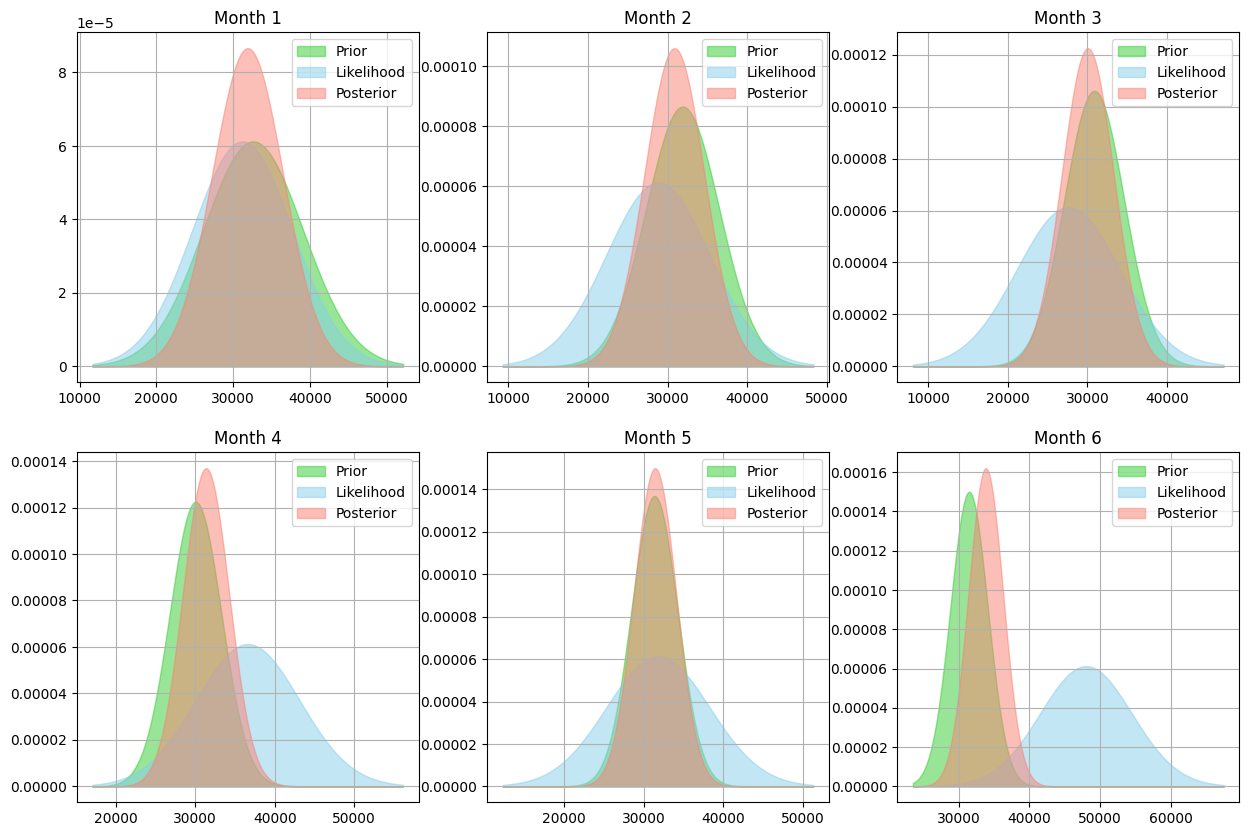
\includegraphics[width=.7\linewidth]{../Report/images/months.png}
  \caption{Prior, Likelihood and Posterior for each month}
\end{figure}

\end{frame}

\begin{frame}{Month-by-Month Posterior Distributions}

  \begin{itemize}
    \item Here, we visualize the evolution of the posterior distributions over each month.
    \item These distributions become more concentrated, indicating increased confidence as more data is incorporated over time.
  \end{itemize}

\begin{figure}
  \centering
  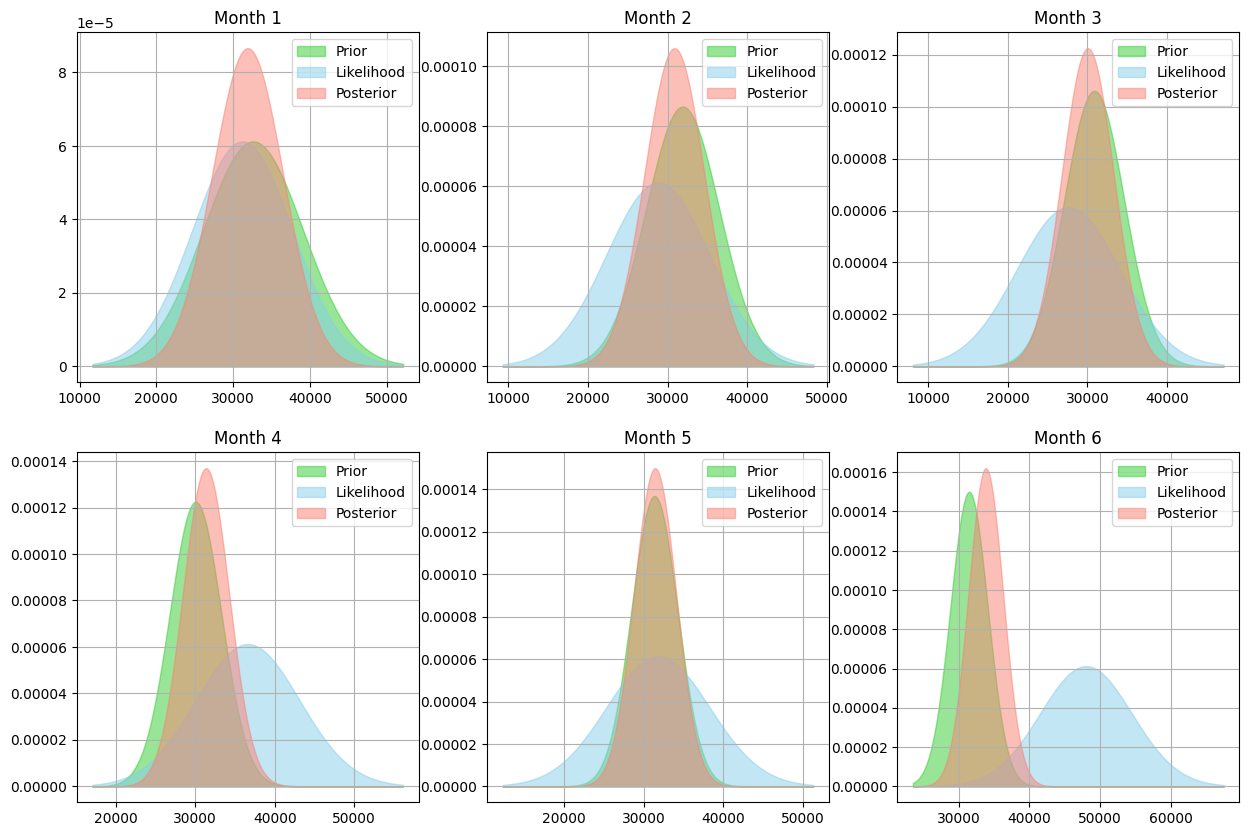
\includegraphics[width=.6\linewidth]{../Report/images/months.png}
  \caption{Posterior Distributions Over Months}
\end{figure}

  
\end{frame}
